\documentclass[11pt]{article}
\usepackage[a4paper,margin=1in]{geometry}
\usepackage{graphicx}
\usepackage{fancyhdr}
\usepackage{titlesec}
\usepackage{listings}
\usepackage{xcolor}
\usepackage{amsmath}
\usepackage{hyperref}

\pagestyle{fancy}
\fancyhf{}
\rhead{STEM Arduino Kit}
\lhead{Experiment 1 Manual}
\rfoot{Page \thepage}

\titleformat{\section}{\normalfont\Large\bfseries}{\thesection}{1em}{}

\definecolor{codegray}{gray}{0.9}
\lstset{
  backgroundcolor=\color{codegray},
  basicstyle=\ttfamily\footnotesize,
  frame=single,
  breaklines=true
}

\begin{document}

\begin{titlepage}
    \centering
    \vspace*{4cm}
    {\Huge \bfseries Measure the Air \par}
    \vspace{1cm}
    {\LARGE STEM Arduino Educational Kit\par}
    \vspace{1cm}
    {\Large Experiment 1: Temperature and Humidity Monitoring with DHT11\par}
    \vfill
    \includegraphics[width=0.5\textwidth]{dht11_diagram.png}\par
    \vspace{2cm}
    {\large \today\par}
\end{titlepage}

\section*{Objective}
Learn how to measure temperature and humidity using sensors, and create a simple temperature alert system with a red LED.

\section*{Materials}
\begin{itemize}
    \item Arduino Uno + USB cable
    \item DHT11 sensor
    \item Breadboard and jumper wires
    \item Red LED and 220$\Omega$ resistor
    \item Computer with Arduino IDE
\end{itemize}

\section*{Circuit Diagram}
\vspace{0.5cm}
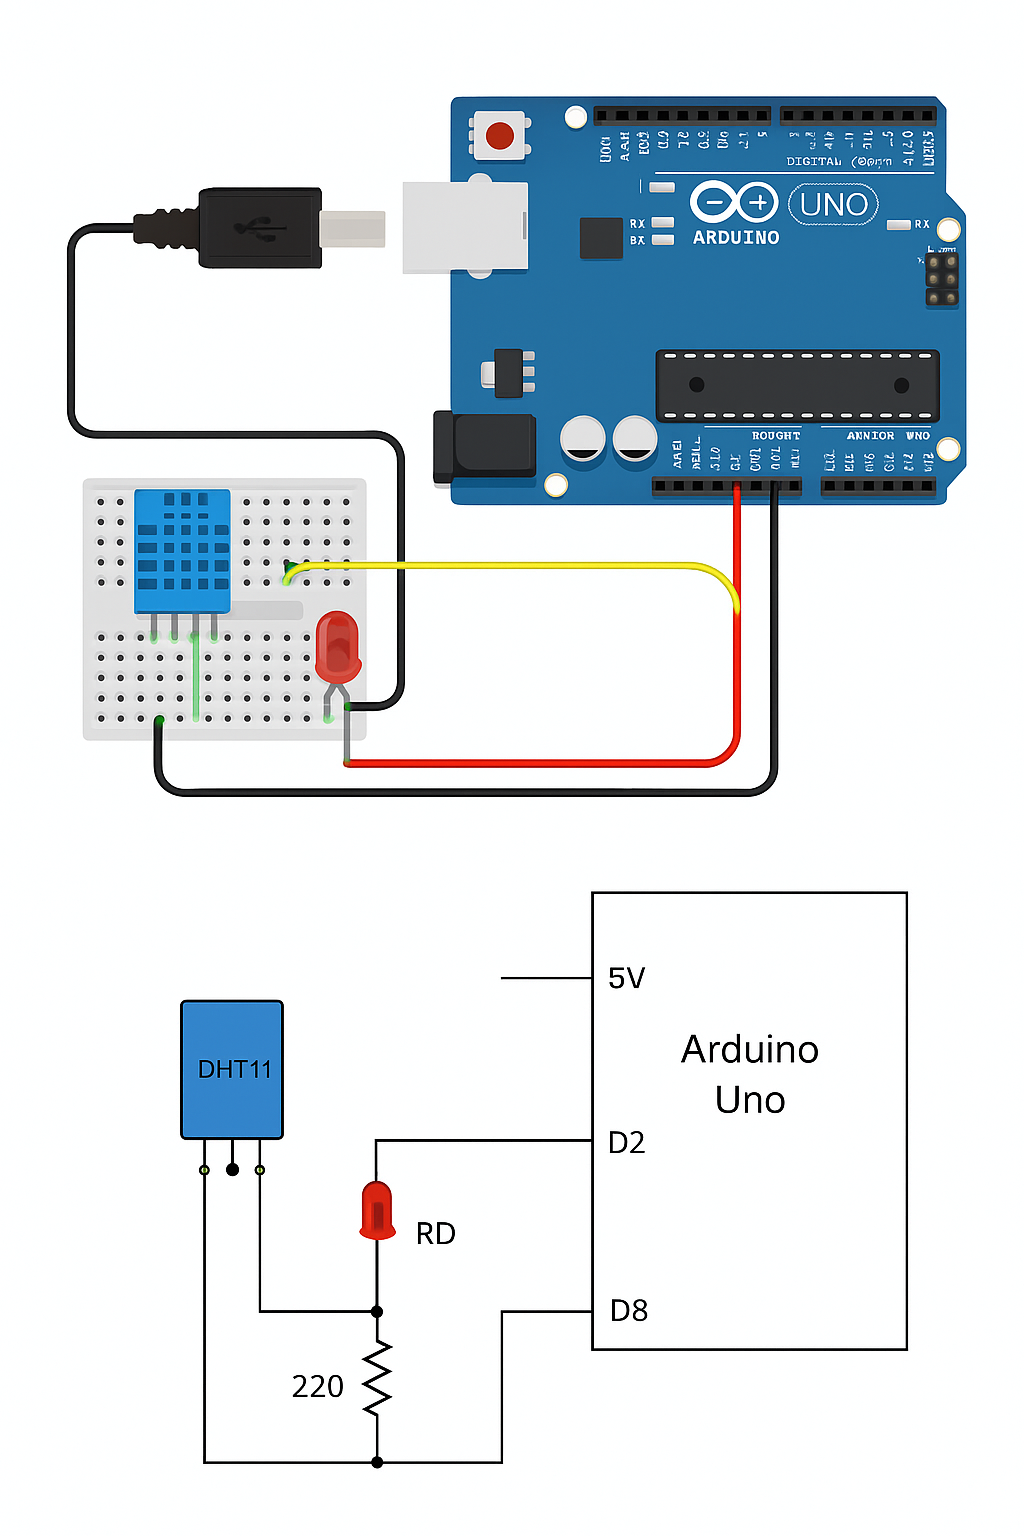
\includegraphics[width=\textwidth]{circuit_diagram_dht11_led.png}
\newline
\textbf{Connections:}
\begin{itemize}
    \item DHT11 VCC $\rightarrow$ 5V on Arduino
    \item DHT11 GND $\rightarrow$ GND
    \item DHT11 DATA $\rightarrow$ D2
    \item LED anode (long leg) $\rightarrow$ D8 via 220$\Omega$ resistor
    \item LED cathode (short leg) $\rightarrow$ GND
\end{itemize}

\section*{Instructions}
\begin{enumerate}
    \item Connect all components as shown in the circuit diagram.
    \item Upload the Arduino code below to your board using the Arduino IDE.
    \item Open the Serial Monitor (magnifying glass icon in the top right).
    \item Observe the temperature and humidity readings printed every 2 seconds.
    \item If the temperature is above 30°C, the LED will turn on.
\end{enumerate}

\section*{Arduino Code}
\lstinputlisting[language=C++, caption=Arduino Sketch for DHT11 + LED]{measure_the_air.ino}

\section*{Learning Outcomes}
\begin{itemize}
    \item Learn how digital sensors work.
    \item Practice reading and interpreting real-world environmental data.
    \item Understand how to use microcontrollers to build alert systems.
\end{itemize}

\section*{Extension Ideas}
\begin{itemize}
    \item Add a buzzer to sound an alarm when it gets too hot.
    \item Log data to an SD card.
    \item Send sensor data via Bluetooth to your mobile phone.
    \item Use a fan to see how fast the temperature changes.
\end{itemize}

\end{document}
